\section{The Sphere Packing Problem}\label{Ch1:Sec:1_1_Sphere_Packing}

The Sphere Packing problem is a classical optimsation problem in mathematics. The problem can be formulated as follows.

\begin{boxproblem}[The Sphere Packing Problem in Dimensinon $n$]\label{Ch1:Prob:SpherePacking_n}
    Given some $n \in \N$, what is the densest possible non-overlapping arrangement of $n$-spheres of equal radius in $\R^n$?
\end{boxproblem}

Despite its rather straightforward formulation, \Cref{Ch1:Prob:SpherePacking_n} is notoriously difficult to solve. Indeed, one obvious question that arises when one looks at the problem statement is how one might define the concept of density. It turns out that the definition is slightly unwieldy, though introducing a periodicity assumption on the sphere packing whose density one wishes to find considerably simplifies this problem.

A key challenge in solving the sphere packing problem in dimension $n$ is the fact that proceeding inductively is not always helpful: `stacking' the optimal $n$-dimensional sphere packing onto itself is not guaranteed to yield the optimal sphere packing in $n + 1$ dimensions.~\cite{CohnOnViazovskaICM}. In fact, this appraoch is known to fail in dimensions as low as $10$~\cite{CohnOnViazovskaAMS}. This is not obvious, not least because the approach does, in fact, succeed in the visualisable dimensions of $1$, $2$ and $3$.

The $1$-dimensional case is uninteresting. Visually, one can easily see that the densest possible arrangement of disjoint intervals of the form $\parenth{-r, r}$ on the real line consists of intervals centred at all points $2rm$ for $m \in \Z$. Indeed, one can fix $r$ to be $\frac{1}{2}$ by rescaling the real line. The optimal packing therefore consists of open intervals of unit length centred at points on the lattice $\Z \subset \R$.

\begin{figure}[htb]
    \centering
    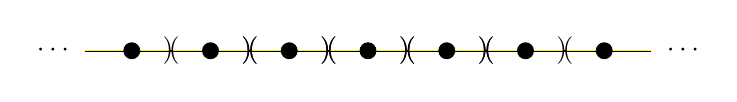
\begin{tikzpicture}
        \draw[step=1, black, thick] (-3.6, 0) -- (3.6, 0);
        \draw[yellow] (-3.6, 0) -- (-2.51, 0);
        \draw[yellow] (2.51, 0) -- (3.6, 0);
        \foreach \x in {-2, -1, 0, 1, 2} {
            \draw[yellow] (\x - 0.49, 0) -- (\x + 0.49, 0);
            \node at (\x - 0.5, 0) {$)\!($};
            \node at (\x + 0.5, 0) {$)\!($};
            \draw[fill=black] (\x, 0) circle (0.1);
        }
        \foreach \x in {-4, 4} {
            \node at (\x,0) {$\cdots$};
        }
        \draw[fill=black] (-3, 0) circle (0.1);
        \draw[fill=black] (3, 0) circle (0.1);
    \end{tikzpicture}
    \caption{The $\Z$ lattice packing in dimension $1$.}
    \label{Ch1:Fig:Z_Lattice_Packing_1D}
\end{figure}

Rescaling gives us a powerful---if straightforward---simplification of the sphere packing problem where we can fix the radius of the spheres to a convenient value. Indeed, we only mention rescaling explicitly because it needs to be explicitly dealt with when formalising the problem. We will resume this discussion in \todo{Add cross-reference}. For now, we will take for granted the fact that rescaling does not affect the density of a sphere packing, meaning that we can talk about optimal sphere packings without worrying about the radius of the spheres in question. Bearing in mind that the spheres must all have the same radius, as per the statement of \Cref{Ch1:Prob:SpherePacking_n}, we will henceforth describe sphere packings simply by describing the points at which the spheres are centred.

The sphere packing problem in dimension $2$, also known as the circle packing problem, turns out to be more interesting. A reasonable strategy for finding the densest packing is to `stack' the $\Z$ lattice packing from dimension $1$ onto itself in some manner, but the question remains as to exactly how this should be done. `Stacking' it onto itself would involve extending the lattice $\Z \subset \R \subset \R^2$ into a lattice in $\R^2$ by extending the $\R$-basis $\set{\parenth{1, 0}}$ of $\R$ (viewed as a subspace of $\R^2$) to an $\R$-basis of $\R^2$, and taking its $\Z$-span.

One natural way of doing this is to extend the lattice $\Z \subset \R$ to the lattice $\Z^2 \subset \R^2$ consisting of points with integer coordinates. This corresponds to the natural extension of $\set{\parenth{1, 0}}$ to the standard $\R$-basis $\set{\parenth{1, 0}, \parenth{0, 1}}$ of $\R^2$. See \Cref{Ch1:Subfig:Z2_lattice_packing_2D}.

Unfortunately, this packing turns out to be sub-optimal \todo{Do we want to add the density?}. A better candidate is the $A_2$ lattice packing, corresponding to the extension of $\set{\parenth{1, 0}}$ to the $A_2$ root basis $\set{\parenth{1, 0}, \parenth{-\frac{1}{2}, \frac{\sqrt{3}}{2}}}$. See \Cref{Ch1:Subfig:A2_lattice_packing_2D}. This packing is sometimes referred to as the \textit{honeycomb packing} due to the fact that every circle has six neighbours, whose centres form the vertices of a regular hexagon.

It is well-known that the honeycomb packing is optimal in $\R^2$. What this means is that no circle packing has a density greater than that of the honeycomb packing. The original proof of this fact is attributed to Thue \cite{Thue}, and it is sometimes referred to in the literature as \textit{Thue's Theorem}. Several other mathematicians have since constructed proofs of Thue's Theorem. One approach based on an idea of Rogers's that does not require particularly sophisticated mathematical tools was outlined by Hales in \cite{CannonHoney}.

\begin{figure}[htb]
    \centering
    \begin{subfigure}{0.48\linewidth}
        \centering
        \begin{tikzpicture}[scale=1.25]
            \drawplane
            \foreach \x in {-2, -1, 0, 1, 2} {
                \foreach \y in {-2, -1, 0, 1, 2} {
                    \latticecircle{\x}{\y}
                }
            }
            \draw[->, color=brown, thick] (0,0) -- (1,0) node[anchor=north] {$\parenth{1, 0}$};
            \draw[->, color=brown, thick] (0,0) -- (0,1) node[anchor=east] {$\parenth{0, 1}$};
        \end{tikzpicture}
        \subcaption{The $\Z^2$ lattice packing.}
        \label{Ch1:Subfig:Z2_lattice_packing_2D}
    \end{subfigure}
    \begin{subfigure}{0.48\linewidth}
        \centering
        \begin{tikzpicture}[scale=1.25]
            \drawplane
            \clip (-2.5, -2.5) rectangle ++(5, 5);
            \foreach \x in {-4, -3, -2, -1, 0, 1, 2, 3, 4} {
                \foreach \y in {-3, -2, -1, 0, 1, 2, 3} {
                    \latticecircle{\x - \y * 0.5}{\y * 0.8660254038}
                }
            }
            \draw[->, color=brown, thick] (0,0) -- (1,0) node[anchor=north] {$\parenth{1, 0}$};
            \draw[->, color=brown, thick] (0,0) -- (-0.5,0.8660254038) node[anchor=south east] {$\parenth{-\frac{1}{2}, \frac{\sqrt{3}}{2}}$};
        \end{tikzpicture}
        \subcaption{The $A_2$ lattice packing.}
        \label{Ch1:Subfig:A2_lattice_packing_2D}
    \end{subfigure}
    \caption{Circle packings covering the square $\setst{\parenth{x, y} \subset \R^2}{-2.5 \leq x, y \leq 2.5}$.}
    \label{Ch1:Fig:Circle_Packings_2D}
\end{figure}

\begin{wrapfigure}[31]{r}{0.27\linewidth}
    \centering
    \begin{subfigure}{\linewidth}
        \centering
        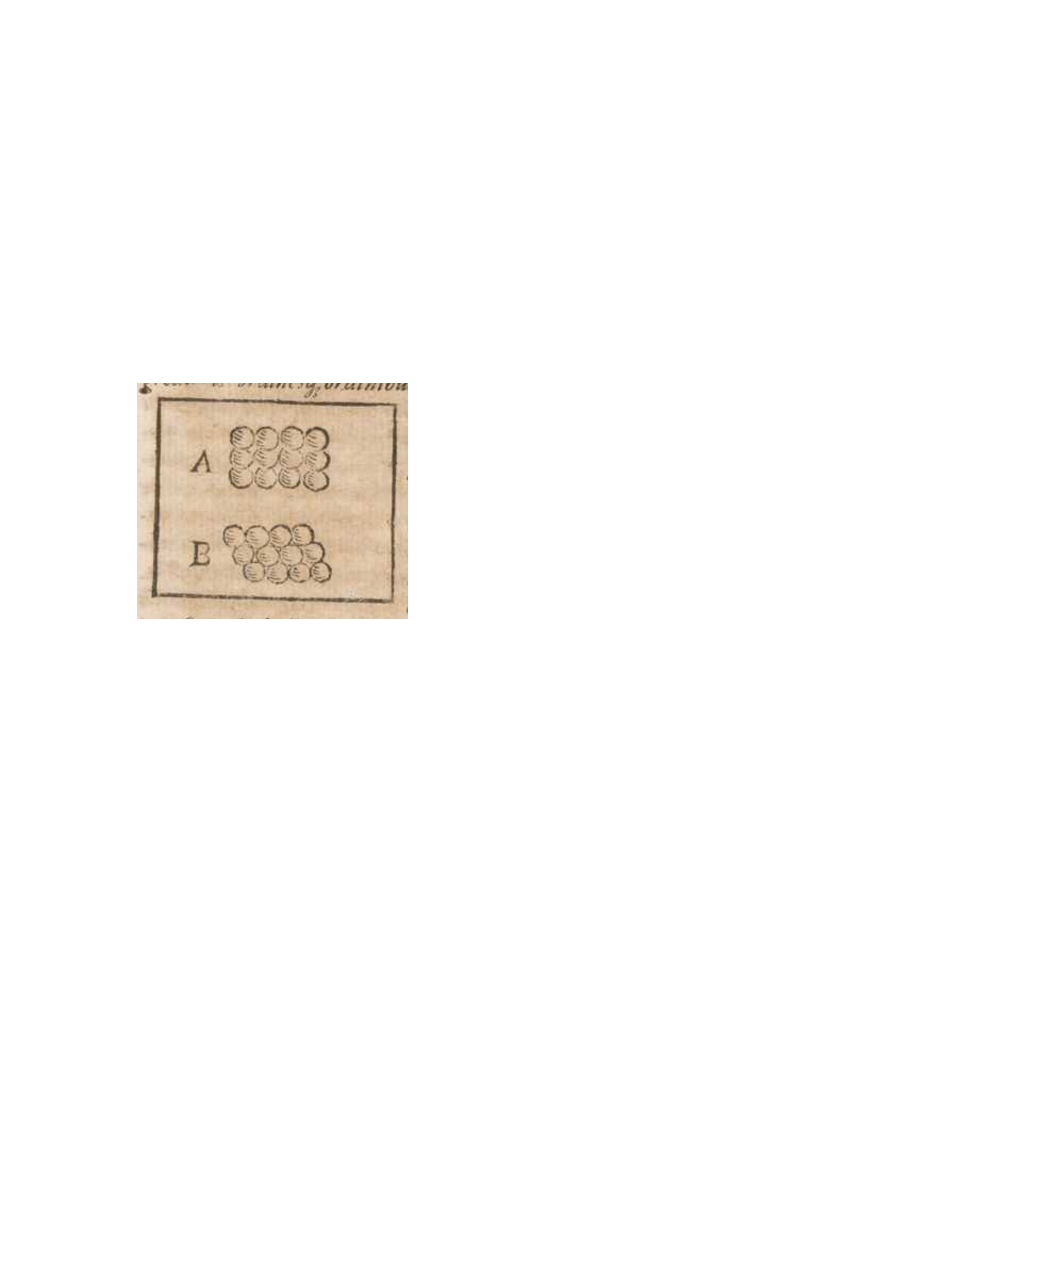
\includegraphics[width=\linewidth]{Chapters/1_Intro/Images/Kepler_1.pdf}
        \caption{}
        \label{Ch1:Subfig:Kepler_Original_1}
    \end{subfigure}
    \begin{subfigure}{\linewidth}
        \centering
        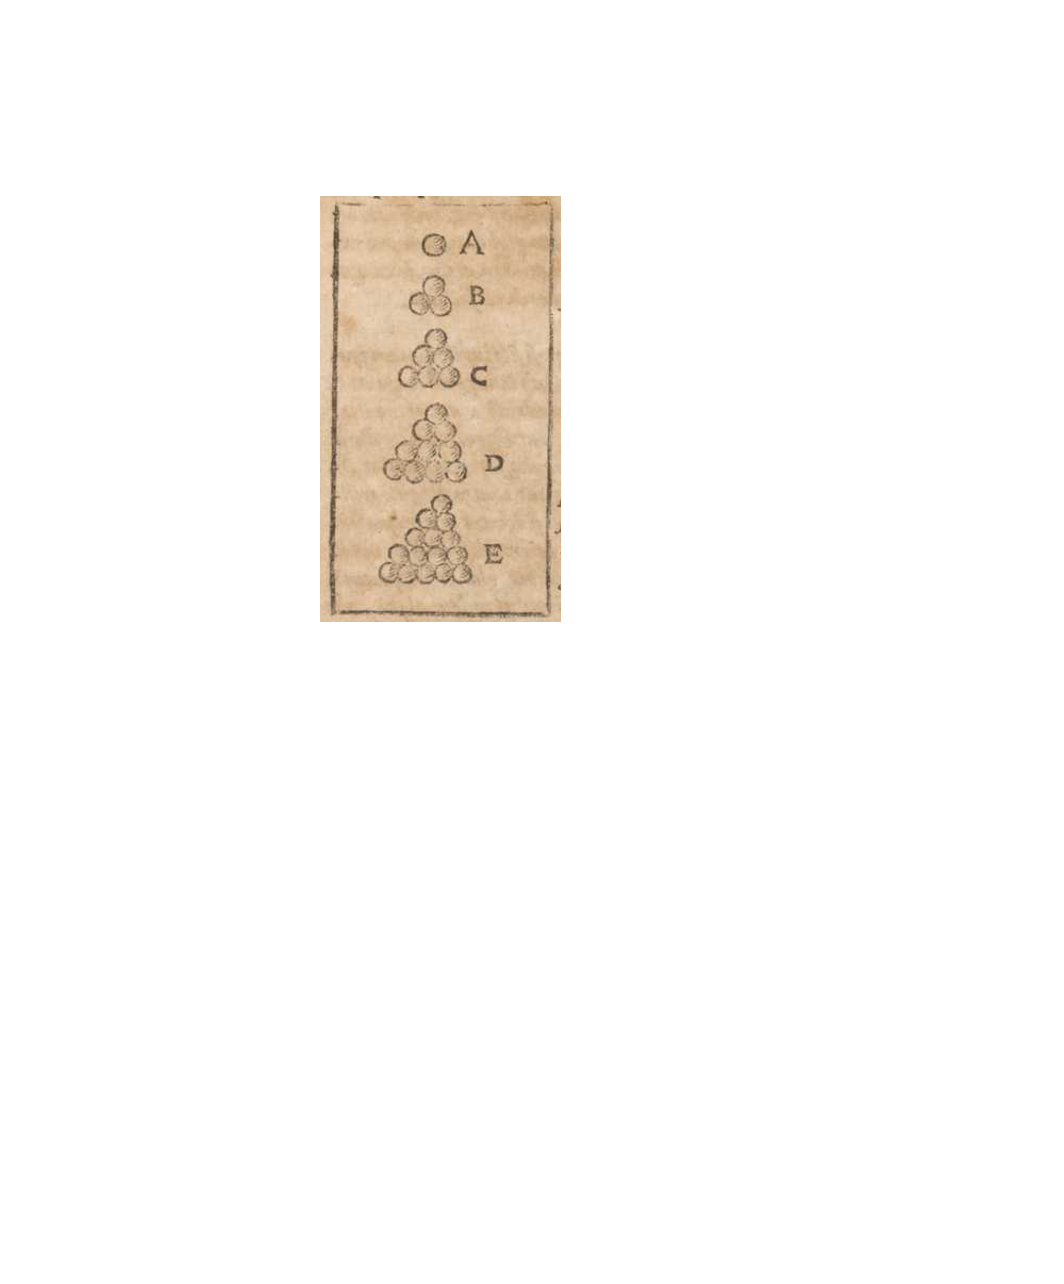
\includegraphics[width=\linewidth]{Chapters/1_Intro/Images/Kepler_2.pdf}
        \caption{}
        \label{Ch1:Subfig:Kepler_Original_2}
    \end{subfigure}
    \caption{Diagrams from an essay written by Johannes Kepler in Latin in 1611 \cite{KeplerSnowflake}.}
\end{wrapfigure}

While we do not offer an exposition of Hales's or any other proof of Thue's Theorem, we include a small discussion of the sphere packing problem in two dimensions to offer some intuition as to why the $A_2$ packing is optimal. For simplicity, we will work under the assumption that the optimal packing in $\R^2$ is some extension of the $\Z$ lattice packing in $\R$, as defined above. We use the strategy of stacking $\Z$ packings on top of each other `row by row', shifting rows around till their density cannot be further increased.

From \Cref{Ch1:Fig:Circle_Packings_2D}, one can convince oneself with relative ease that the $A_2$ packing is denser than the $\Z^2$ packing. This makes it denser than any packing that is sparser than the $\Z^2$ packing. In particular, we only need to improve the $\Z^2$ packing to construct the optimal packing. Since vertical shifts only push rows further apart, rendering the packing sparser, it suffices to consider horizontal row shifts. In the $\Z^2$ packing, each circle in a given row is in contact with only one sphere from the row below. A natural improvement is to shift rows about so each circle is in contact with \textit{two} circles from the row below. This results in the $A_2$ lattice packing. This packing cannot be improved because it is impossible for a circle to be in contact with \textit{three} circles from the row below due to the separation between circles in the one-dimension $\Z$ packing. See \Cref{Ch1:Subfig:Kepler_Original_1}.

While this is far from a rigorous argument, this approach illustrates why we should not be surprised that the $A_2$ sphere packing is optimal: the key observation is that the $A_2$ packing maximises the number of neighbours a circle can have. Admittedly, it is neither obvious why this optimises density nor why the optimal packing involves stacking the $\Z$ packing repeatedly on itself, not least because we have yet to formally define the density of a sphere packing. We merely reassure the reader, at this stage, that the definitions and characteristics of the sphere packing problem in $\R^2$ strongly agree with visual intuition. With this, we close our discussion.

In dimension $3$, too, it is tempting to replicate this strategy: we can attempt to stack the $A_2$ packing on top of itself, in layers instead of rows, in such a manner as maximises the number of neighbours a sphere can have. From trial and error, it appears to be the case that a sphere cannot be in contact with more than three neighbours from the layer below. This suggests that the optimal sphere packing in dimension $3$ is given by stacking honeycomb arrangements on top of each other with spheres in each layer being nestled in the gaps between three spheres in the layer below.

As it turns out, unlike dimension $2$, a characterisation in terms of the number of neighbours in the layer below does not describe a unique packing. In $\R^3$, spheres are so large that it is not possible to stack honeycomb arrangements on top of each other such that \textit{all} gaps between spheres in one layer are occupied by spheres in the next. There is no unique stacking of honeycomb layers such that each sphere has exactly three neighbours in the layer below: in different stackings, the spheres in a layer might fill a different arrangement of gaps between spheres in the layer below, as shown in \Cref{Ch1:Fig:2_Optimal_3D_Packings}. One can construct many different sphere packings in $\R^3$, all of which are as dense as possible, by varying how successive layers are placed. For instance, the sphere packing obtained by successively repeating the arrangement in \Cref{Ch1:Subfig:3D_Triangular_Stacking} and that obtained by alternating between the arrangements in \Cref{Ch1:Subfig:3D_Triangular_Stacking} and \Cref{Ch1:Subfig:3D_Hexagonal_Stacking} are globally different, despite having the same density and identical layers. The former is referred to as the \textit{face-centred cubic packing} and the latter is referred to as the \textit{hexagonal close-packing}.

\begin{figure}[htb]
    \centering
    \begin{subfigure}{0.48\linewidth}
        \centering
        \begin{tikzpicture}[scale=1.25]
            \clip (-2.5, -2.5) rectangle ++(5, 5);
            \foreach \x in {-4, -3, -2, -1, 0, 1, 2, 3, 4} {
                \foreach \y in {-3, -2, -1, 0, 1, 2, 3} {
                    \latticecircle{\x - \y * 0.5}{\y * 0.8660254038}
                }
            }
            \foreach \x in {-3, -2, -1, 0, 1, 2} {
                \foreach \y in {-3, -2, -1, 0, 1, 2} {
                    \latticecirclegrey{\x - \y * 0.5}{\y * 0.8660254038 + 0.5773502692}
                }
            }
        \end{tikzpicture}
        \subcaption{}
        \label{Ch1:Subfig:3D_Triangular_Stacking}
    \end{subfigure}
    \begin{subfigure}{0.48\linewidth}
        \centering
        \begin{tikzpicture}[scale=1.25]
            \clip (-2.5, -2.5) rectangle ++(5, 5);
            \foreach \x in {-4, -3, -2, -1, 0, 1, 2, 3, 4} {
                \foreach \y in {-3, -2, -1, 0, 1, 2, 3} {
                    \latticecircle{\x - \y * 0.5}{\y * 0.8660254038}
                }
            }
            \foreach \x in {-2, -1, 0, 1, 2, 3} {
                \foreach \y in {-2, -1, 0, 1, 2, 3} {
                    \latticecirclegrey{\x - \y * 0.5}{\y * 0.8660254038 - 0.5773502692}
                }
            }
        \end{tikzpicture}
        \subcaption{}
        \label{Ch1:Subfig:3D_Hexagonal_Stacking}
    \end{subfigure}
    \caption{Two different ways of stacking the honeycomb packing on itself.}
    \label{Ch1:Fig:2_Optimal_3D_Packings}
\end{figure}

The face-centred cubic packing can be visualised by thinking about how spheres can be arranged tetrahedrally. For some $n$, let $T_n := n\parenth{n + 1}/2$ be the $n$th triangular number\footnote{See \href{https://oeis.org/A000217}{OEIS A000217}}. Begin by arranging $T_n$ spheres in a triangular formation. On top of this layer, arrange $T_{n - 1}$ spheres in a triangular formation, such that each sphere is nestled in the gaps between the spheres in the layer below, as in \Cref{Ch1:Subfig:3D_Triangular_Stacking}. Continue in this manner till there is only one ball left to be arranged. This leads to an arrangement in which the number of spheres is the $n$th tetrahedral number\footnote{See \href{https://oeis.org/A000292}{OEIS A000292}}. A key characteristic of the face-centred cubic packing is that it consists of such arrangements. In fact, in a 1611 essay whose title has been translated from Latin as \textit{The Six-Cornered Snowflake} \cite{KeplerSnowflake}, it was asserted by Johannes Kepler that spheres cannot be more tightly packed together than they are in a tetrahedral arrangement. This assertion was accompanied by an illustration: see \Cref{Ch1:Subfig:Kepler_Original_2}. For over three centuries, this assertion remained unproven, and was referred to as the \textit{Kepler Conjecture}. It was only in 2005 that a paper proving the Kepler Conjecture, written by Thomas Hales, was published \cite{HalesKeplerInformal}.

The complexity of the sphere packing problem in dimension $3$ is illustrated not only by the time elapsed between Kepler's original assertion and a proof being published but also by the length of Hales's paper. Indeed, in an expository account of his proof published in 2000, five years before the publication of the full paper in the Annals, Hales recounted how a jury of twelve referees, despite having been in deliberation for over a year, had yet to make a ``thorough, independent check of the computer code'' he had written to perform the elaborate calculations on which ``every aspect of [his proof] is based'' \cite{CannonHoney}. In January 2003, at the Joint Math Meetings in Baltimore, USA, Hales announced that he intended to formally verify his proof \cite{HalesKeplerFormal}. The paper authored by Hales and his collaborators on their successful formalisation of his argument was only published in 2017. Therefore, not only did the Kepler Conjecture take close to 400 years to solve, but it took nearly two decades to eliminate any doubt as to the correctness of the solution.

At first glance, this appears to set a dangerous precedent for the sphere packing problem in other dimensions. It well might, for there is much we do not understand about the behaviour of spheres in high dimensions. In the words of Henry Cohn, ``each dimension has its own idiosyncracies and charm" \cite{CohnOnViazovskaAMS}. That being said, in the specific cases of dimensions $8$ and $24$, this turns out to work in our favour.

The solutions in dimensions $8$ and $24$ are products of the same recipe, which consists primarily of two ingredients. The first is a linear programming bound from a 2003 paper by Henry Cohn and Noam Elkies \cite[Theorem 3.1]{CohnElkies} on all sphere packing densities in $\R^n$. The second is the remarkable insight that the theory of modular forms can be used to obtain tight bounds in dimensions $8$ and $24$, equal to the densities of the $E_8$ and Leech lattice packings respectively.

The applicability of the theory of modular forms comes from the formulation of Cohn and Elkies's theorem: if a function $f : \R^n \to \R$ satisfies certain conditions, then \textit{all} sphere packings in $\R^n$ are bounded above by a quantity that depends on $f$. The trick is therefore not only to find a function satisfying the Cohn-Elkies conditions but to find one for which the Cohn-Elkies bound also corresponds to the density of some sphere packing in $\R^n$. Viazovska's groundbreaking contribution was constructing such a function in dimension $8$ using the theory of modular forms. The function is often referred to as the Magic Function, a term we shall adopt in this project because it befits the nature of Viazovska's achievement. A similar approach was used in dimension $24$ by Cohn, Kumar, Miller, Radchenko and Viazovska.

As tempting as it is to continue our discussion on the sphere packing problem, this project does consist of two parts: a mathematical examination of the construction of Viazovska's Magic Function in dimension $8$ and a formalisation thereof. We will therefore pause this discussion and take a detour into the world of formalisation, which will offer context for the second part of this project.